\chapter{Nelson e Kay}

\section{Verso gli ipertesti: Ted Nelson}

Ted Nelson nacque nel 1937, i suoi genitori (un'attrice e un regista) divorziarono nel 1939 e lui venne cresciuto dai nonni
materni. Nelson studiò filosofia e si laureò in sociologia (1963) prendendo un dottorato nel 
2002 (in realtà la sua tesi è una riproposizione di idee avute nel 1959).
Le sue pubblicazioni più importanti sono:

\begin{itemize}
    \item [$\Rightarrow$] \fancyglitter{Complex Information Processing: A File Structure for the Complex, the Changing and the Indeterminate} (1965): 
    articolo tecnico in cui si introduce il concetto di \fancyglitter{ipertesto} con le strutture dati collegate;
    \item [$\Rightarrow$] \fancyglitter{Computer Lib/Dream Machines} (1974): libro autopubblicato.
    Il titolo è doppio perché il libro è doppio, ossia si legge in due direzioni.
    Inoltre la grafica richiama una pubblicazione della controcultura hippie (curata da Stewart Brand),
    ossia il \fancyglitter{Whole Earth Catalog}\footnote{Catalogo di oggetti (in particolar modo libri)
    messi in vendita. Molti testi appartenevano alla libreria dello Xerox PARC.};
    \item [$\Rightarrow$] \fancyglitter{Literary Machines} (1981): descrizione del sistema Xanadu.
\end{itemize}

\clm{}{}{
    Nelson fa il compleanno lo stesso giorno del prof. Cardone.
}

\clm{}{}{

\paragraph{Nelson ha anche girato un video "estremo":}

\begin{itemize}
    \item [$\Rightarrow$] \fancyglitter{Silicon Valley Story} (1992): non si capisce niente, surreale. Ma compaiono personaggi come 
    Timoty Leary (profeta delle droghe psichedeliche\footnote{AKA psicologo di Harvard.}), Douglas Engelbart e Stuart Brand.
\end{itemize}
}

\subsection{Xanadu e Parallel Textface}

Anche Nelson fa parte del gruppo di persone che ha letto \fancyglitter{As We May Think} di Vannevar Bush.
Nelson scrive un articolo, \fancyglitter{As We Will Think}, dove analizza il testo di Bush. 

\paragraph{Per Nelson il memex può essere considerato come:}

\begin{itemize}
    \item [$\Rightarrow$] Una console personale per la \fancyglitter{presentazione}, la 
    \fancyglitter{manipolazione} (editing) e l'\fancyglitter{archiviazione} (file);
    \item [$\Rightarrow$] Una \fancyglitter{rete di alimentazione per la distribuzione di documenti} in formato digitale\footnote{Bush pensava alla condivisione su microfilm.};
    \item [$\Rightarrow$] Un \fancyglitter{nuovo tipo di documento} (ipertesto), pensato per essere ricevuto e spedito.
\end{itemize}

\subsubsection{}

In As We Will Think Nelson parla delle interpretazioni sbagliate che sono 
state date all'articolo di Bush. Per esempio un interesse di Bush nel rendere 
più efficiente l'indicizzazione (Information retrieval) che in realtà non c'era.
Come abbiamo visto il memex è in contrasto con tutto ciò.
Nel \fancyglitter{sistema Xanadu} Nelson spiega la sua interpretazione del 
memex e delle idee di Bush.

\dfn{Xanadu}{
    Xanadu è un sistema stand-alone, costruito su un minicomputer con vari 
    metodi di recupero delle informazioni automatici e manipolazione del database del 
    sistema soggiacente tramite \newfancyglitter{theaters} (front-end).
}

\cor{Parallel Textface}{
    Il più importante dei theaters è il \fancyglitter{Parallel Textface}: un 
    sistema testuale di una certa potenza e raffinatezza.

    L'utente siede davanti allo schermo con una tastiera o una lightpen 
    e può scrivere, cancellare, spostare, copiare e incollare testo. La 
    memorizzazione è digitale.
}

\nt{Il Parallel Textface è un'implementazione delle "note e commenti marginali" di Bush.}

\subsection{Ipertesti}

Nel 1967, Nelson scrisse delle note\footnote{Mai pubblicate.} significative sugli ipertesti.

\clm{}{}{Le sue note si possono trovare nell'archivio di Nelson. Purtroppo
Nelson è molto disordinato quindi molte delle sue note sono incomprensibili fuori dal contesto,
scarabocchi su carta, etc.}

\begin{figure}[h]
    \centering
    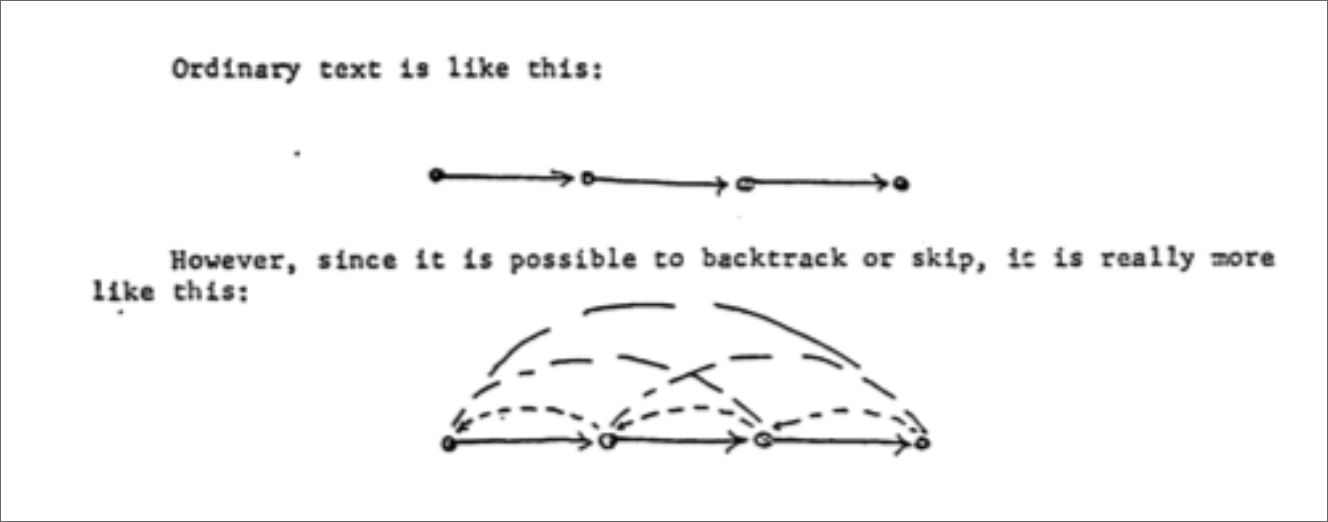
\includegraphics[scale=0.35]{images/H1.png}
\end{figure}

\begin{figure}[h]
    \centering
    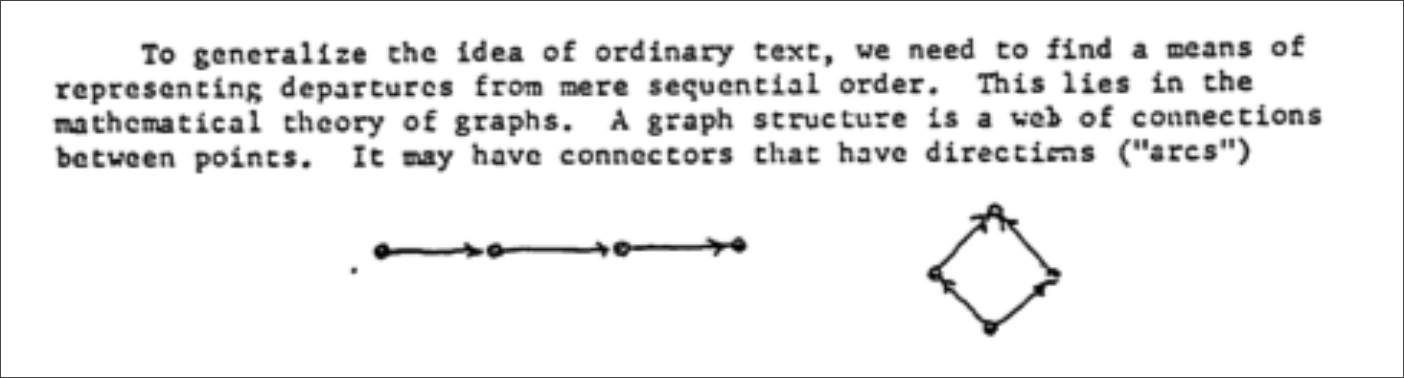
\includegraphics[scale=0.25]{images/H2.png}
    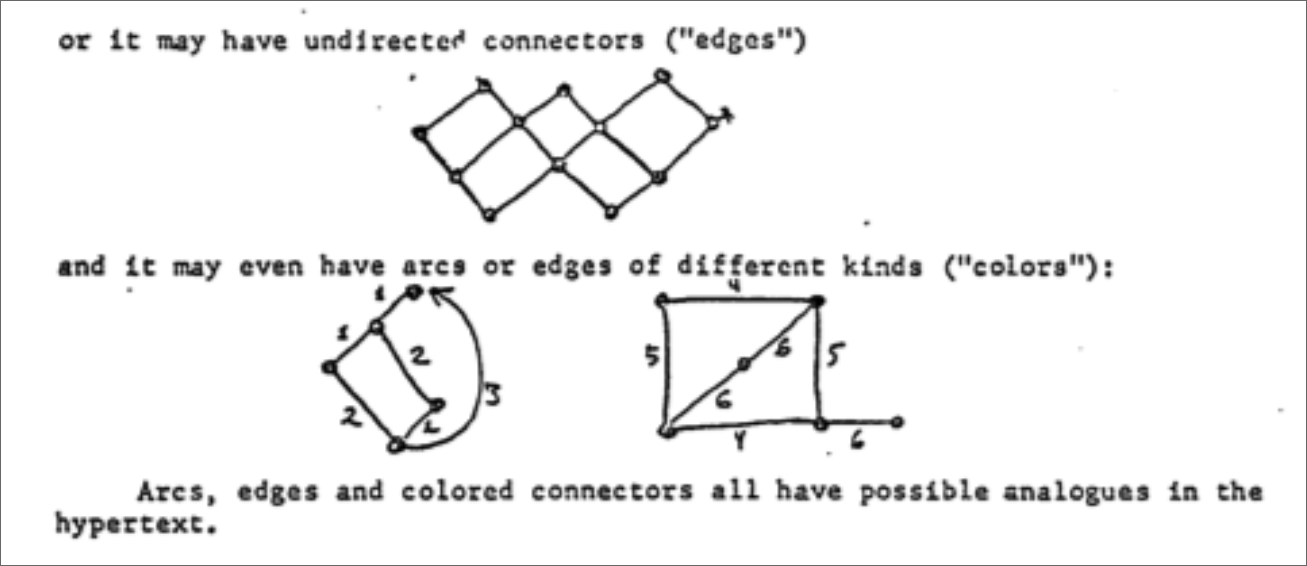
\includegraphics[scale=0.25]{images/H3.png}
\end{figure}

\nt{Un esempio di ipertesto come inteso da Nelson sono 
le mappe mentali o le mappe concettuali.
}

\clm{}{}{
    Engelbart, al contrario di Nelson, era più un fan dei testi strutturati
    ad albero diviso in capitoli, sezioni, sottosezioni,
    etc. dove sono le etichette a stabilire dei link tra parti 
    diverse di un testo (Un po' come i miei appunti).
}

\dfn{Connettori}{
    Si hanno due tipi di \newfancyglitter{annotazioni} (connettori):
    \begin{itemize}
        \item [$\Rightarrow$] \fancyglitter{Tag}: marcatore nel testo a cui
        è allegata una breve nota o spiegazione;
        \item [$\Rightarrow$] \fancyglitter{Link}: collegamento tra due elementi testuali. 
        È un salto da un punto a un altro. 
    \end{itemize}
}

\dfn{Piste}{
    La \fancyglitter{pista} (trail) è una sequenza di documenti, estratti
    di documenti e commenti su essi. Si stabilisce realizzando degli accoppiamenti.
}

\cor{Tipi di piste}{
    \begin{itemize}
        \item [$\Rightarrow$] \fancyglitter{Side trail}: pista laterale,
        si dirama da una pista principale;
        \item [$\Rightarrow$] \fancyglitter{Skip trail}: sottoinsieme 
        di una pista principale, contiene solo i punti salienti.
    \end{itemize}
}

\clm{}{}{
    Tutto ciò che si fa in questo corso è opinabile e soggetto a eventuali critiche.
    È necessario riflettere su queste cose, per esempio: in un ipertesto, che 
    nasce per contrastare la struttura sequenziale, bisogna comunque tracciare delle 
    piste, ricadendo nell'inevitibilità della sequenzialità.

    La critica di Nelson al testo sequenzializzato è a sua volta criticabile.
}

\qs{}{Ma quindi che cos'è, per Nelson, un ipertesto?}

\dfn{Ipertesto}{
    Un ipertesto è una struttura del testo che non può essere comodamente
    stampata.
}

\cor{Stretchtext}{
    Un esempio di ipertesto è lo \fancyglitter{stretchtext}, un testo che 
    può essere allungato a piacimento.
}

\nt{Interi ipertesti possono essere collegati tra loro formando dei libri.
Idee già viste nella classificazione di Otlet, nelle biblioteche del futuro di Licklider e 
nel memex di Bush.}

\dfn{Transclusion}{
    La \newfancyglitter{transclusion} è un'operazione che permette di condividere fisicamente
    un testo in altri testi.
}

\cor{Collateration}{
    La \fancyglitter{collateration} è un'operazione che permette di creare collegamenti
    con \fancyglitter{zippered lists} (liste con cerniere) per mezzo di link visualizzabili.
}

\begin{figure}[h]
    \centering
    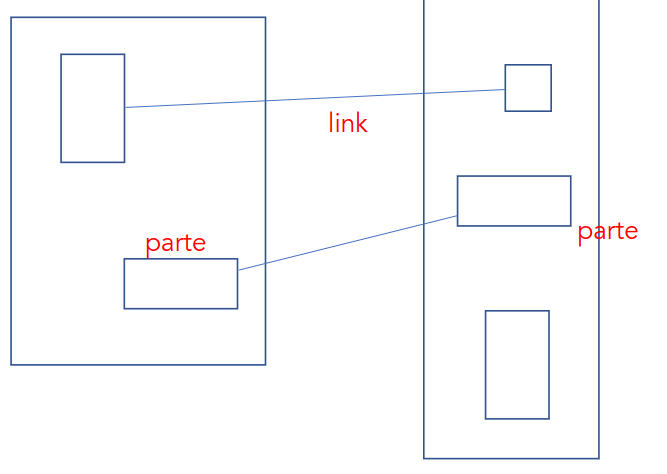
\includegraphics[scale=0.45]{images/Col.png}
\end{figure}

\nt{Esempi di collateration sono le note a margine, le note a piè di pagina, sommari, indici, intestazioni, etc.

Ossia il paratesto.}

\dfn{Docuverso}{
    Il \newfancyglitter{docuverso} è un nuovo sistema di iperpubblicazione che
    contiene un insieme di documenti collegati tra loro, grazie alla transclusion.

    Questo è alla base di Xanadu.
}

\subsection{Implemetazione degli ipertesti}


\begin{itemize}
    \item [$\Rightarrow$] \fancyglitter{Pianificazione di strutture non lineari}: per esempio delle mostre;
    \item [$\Rightarrow$] \fancyglitter{Strutture informative in forma grafica}: per esempio diagrammi PERT e programmi;
    \item [$\Rightarrow$] \fancyglitter{Hypermedia}: per esempio alcuni film, fumetti, etc.
\end{itemize}

\dfn{NoteCards}{
    Le \newfancyglitter{NoteCards} sono un sistema di Hypermedia per 
    rappresentare e manipolare informazioni. Sono state sviluppate a 
    Xerox PARC.
}

\ex{NoteCards}{
    \begin{center}
        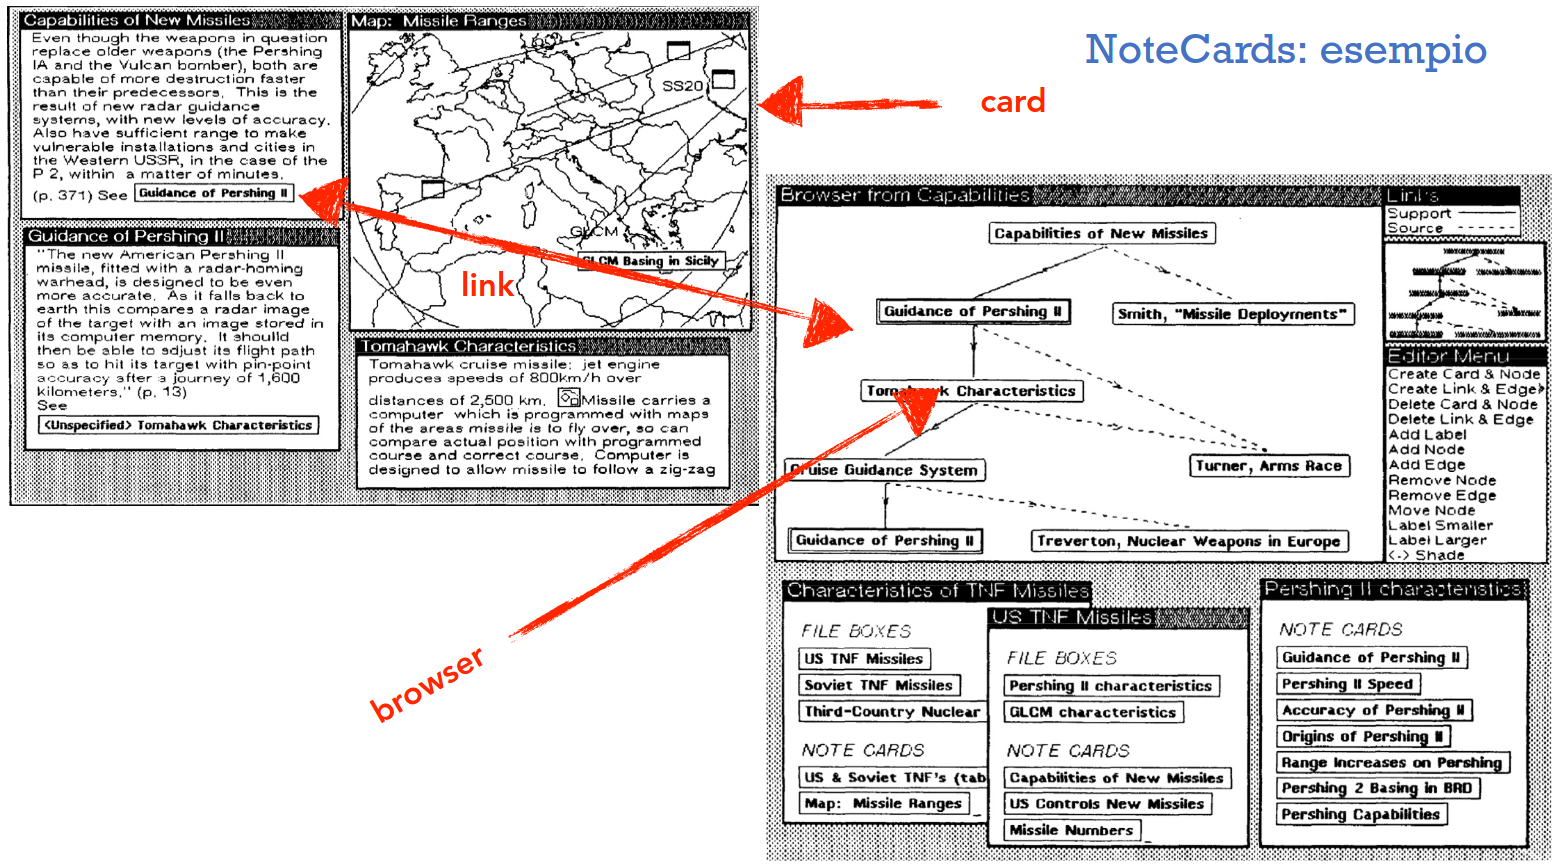
\includegraphics[scale=0.25]{images/NC.png}
    \end{center}
}

\nt{Successivamente si può parlare di HyperCard, che veniva regalato con i Macintosh.
HyperCard è un sistema di pile di schede e aveva una funzione didattica.}

\dfn{Thinkertoys}{
    I \newfancyglitter{Thinkertoys} sono un sistema di visualizzazione
    per computer che aiuta a considerare alternativa complesse.
}
\paragraph{Alternative complesse:}
\begin{itemize}
    \item [$\Rightarrow$] Progetti alternativi;
    \item [$\Rightarrow$] Discrepanze tra le testimonianze;
    \item [$\Rightarrow$] Bozze successive di un documento.
\end{itemize}

\dfn{Fantics}{
    La \newfancyglitter{fantics} (o fantica) è:
    \begin{itemize}
        \item [$\Rightarrow$] L'arte e la scienza della presentazione;
        \item [$\Rightarrow$] Tecniche di presentazione: scrittura, regia, realizzazione di filmati, etc.
        \item [$\Rightarrow$] I media, la loro analisi, la loro progettazione, etc.;
        \item [$\Rightarrow$] La progettazione di sistemi per le presentazioni.
    \end{itemize}
    
}

\nt{Nelson parla di spazio fantico: uno spazio creato ad arte per la 
presentazione di informazioni. Da ricordare la figura del 
"Facilitatore visuale" nata nel laboratorio di Engelbart.}

\section{Il Computer come Medium: Alan Kay}

Alan Kay è nato nel 1940. Dal punto di vista della storia dell'informatica è importante perché creò lo Smalltalk\footnote{Visto nella prima parte del corso.}
Nel 1962 si arruola nell'esercito e analizza il sistema per condividere i dati tra basi militari:

\begin{itemize}
    \item [$\Rightarrow$] La prima parte era una \fancyglitter{sequenza di puntatori} alla seconda parte;
    \item [$\Rightarrow$] La seconda parte conteneva le \fancyglitter{procedure} utilizzate per accedere e modificare i dati della terza parte;
    \item [$\Rightarrow$] La terza parte conteneva i \fancyglitter{record} con i dati.
\end{itemize}

\begin{figure}[h]
    \centering
    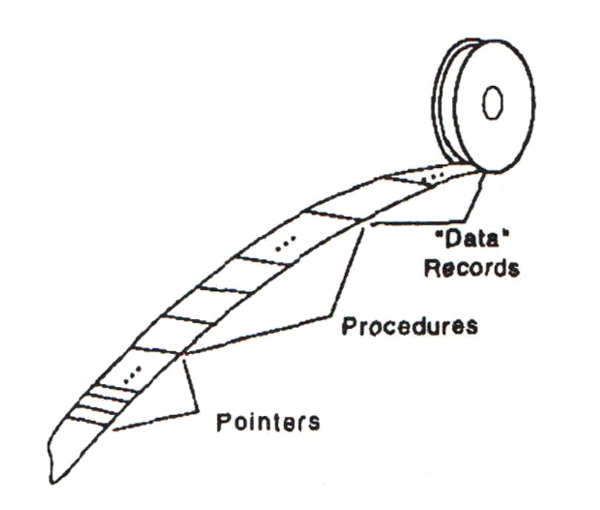
\includegraphics[scale=0.5]{images/Data.png}
\end{figure}
\pagebreak
\subsection{Gli inizi}

Dopo la laurea Kay entra nel programma di dottorato\footnote{Era stato creato da poco grazie a Licklider.} all'università di Utah.
Qua scopre \fancyglitter{Sketchpad} (programma di grafica interattiva) di Ivan Sutherland.

\dfn{Simula 67}{
    Il \newfancyglitter{Simula 67} è un linguaggio di programmazione orientato agli oggetti
    inventato da Ole-Johan Dahl e Kristen Nygaard.
}

\paragraph{Kay osservò le relazioni tra Sketchpad e Simula 67 (con una metafora biologica):}

\begin{itemize}
    \item [$\Rightarrow$] Le cellule ("instances") si conformano ai comportamenti "master";
    \item [$\Rightarrow$] Le cellule sono autonome e comunicano tra loro scambiandosi messaggi;
    \item [$\Rightarrow$] Le cellule diventano parti diverse di un organismo a seconda del contesto.
\end{itemize}

\nt{Questa metafora sarà alla base del Smalltalk.}

\paragraph{Altre influenze che hanno dato forma al lavoro di Kay:}

\begin{itemize}
    \item [$\Rightarrow$] \fancyglitter{McLuhan}: il medium è il messaggio;
    \item [$\Rightarrow$] \fancyglitter{Papert e il linguaggio LOGO}\footnote{Visti nel corso "Metodologie
    e Tecnologie Didattiche per l'Informatica".}: il computer come strumento per l'apprendimento.
\end{itemize}

\begin{figure}[h]
    \centering
    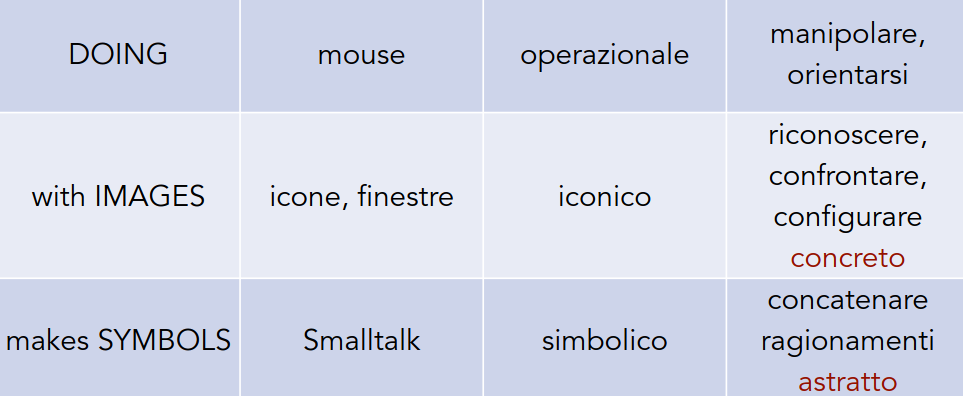
\includegraphics[scale=0.45]{images/App.png}
    \caption{Apprendimento secondo Kay.}
\end{figure}


\subsection{Il Dynabook}

\nt{Il computer è un medium di comunicazione:
\begin{itemize}
    \item [$\Rightarrow$] Conversazionale;
    \item [$\Rightarrow$] Attivo;
    \item [$\Rightarrow$] Universale: può essere usato per simulare qualsiasi altro media;
    \item [$\Rightarrow$] Dinamico.
\end{itemize}
}

\dfn{Dynabook}{
    Il \newfancyglitter{Dynabook} è un computer portatile per bambini, con un'interfaccia grafica e un linguaggio di programmazione semplice.
}

\nt{Non molto diverso da un tablet.}

\begin{figure}[h]
    \centering
    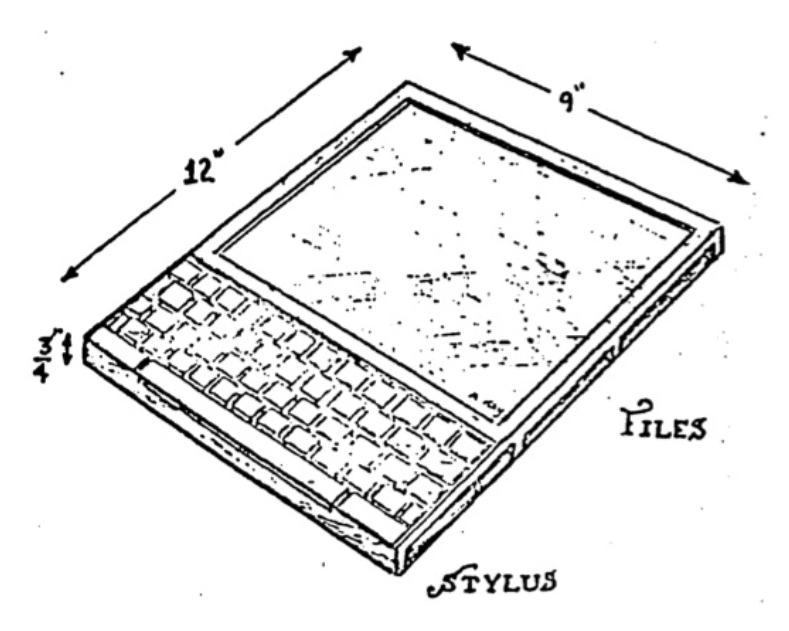
\includegraphics[scale=0.45]{images/Dyn.png}
    \caption{Il Dynabook.}
\end{figure}

\paragraph{Caratteristiche del Dynabook:}

\begin{itemize}
    \item [$\Rightarrow$] Possibilità di memorizzazione interattiva;
    \item [$\Rightarrow$] Lettura di testi ordinari e ipertesti;
    \item [$\Rightarrow$] Fonts personalizzabili;
    \item [$\Rightarrow$] WYSIWYG\footnote{
        What You See Is What You Get: il testo visualizzato sullo schermo è uguale a quello stampato.
    } nell'editing di testi;
    \item [$\Rightarrow$] Finestre multiple e sovrapponibili;
    \item [$\Rightarrow$] Sensorializzazione di processi dinamici;
    \item [$\Rightarrow$] Animazione e musica;
    \item [$\Rightarrow$] Programmazione;
    \item [$\Rightarrow$] Simulazione.
\end{itemize}

\dfn{Xerox ALTO}{
    L'Xerox ALTO\footnote{Visto nella prima parte del corso.} è un tentativo di realizzare il Dynabook.
}

\dfn{Xerox NoteTaker}{
    Il \newfancyglitter{Xerox NoteTaker} fu il primo computer portatile utilizzato in aereo da 
    Douglas Fairbairn (informatico che si occupò di linguaggi funzionali).
}

\subsection{Smalltalk}

\dfn{Smalltalk}{
    Lo \newfancyglitter{Smalltalk} è un linguaggio di programmazione orientato agli oggetti
    che avrebbe dovuto essere usato per programmare il Dynabook.
}

\paragraph{Principi dello Smalltalk:}

\begin{itemize}
    \item [$\Rightarrow$] \fancyglitter{Oggetti}: tutto è un oggetto;
    \item [$\Rightarrow$] \fancyglitter{Messaggi}: gli oggetti comunicano scambiandosi messaggi (oggetti);
    \item [$\Rightarrow$] Gli oggetti hanno \fancyglitter{memoria privata};
    \item [$\Rightarrow$] Ogni oggetto è istanza di una \fancyglitter{classe};
    \item [$\Rightarrow$] Le classi contengono i \fancyglitter{comportamenti} comuni alle loro istanze;
    \item [$\Rightarrow$] Per valutare un programma il controllo è passato al primo oggetto e il resto è 
    interpretato come un suo messaggio.
\end{itemize}

\begin{figure}[h]
    \centering
    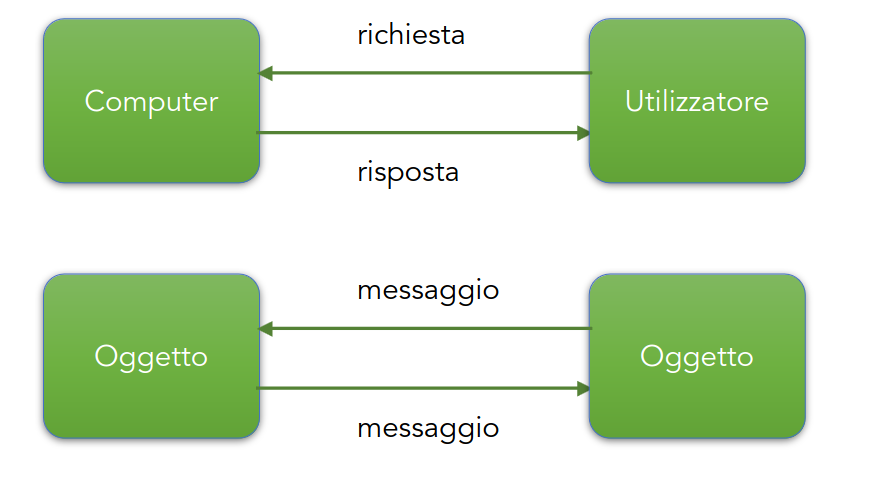
\includegraphics[scale=0.5]{images/Small.png}
    \caption{Smalltalk.}
\end{figure}


\section{Per concludere: una storia alternativa}

\subsection{Whole Earth Catalog e Computer Lib/Dream Machines}

Il \fancyglitter{Whole Earth Catalog} fu una pubblicazione curata da Stewart Brand.
Si trattava di un catalogo di oggetti (in particolar modo libri) messi in vendita, con 
al centro il motto "Access to tools", garantendo l'accesso a strumenti e conoscenze.
Si trattava di un'opera di controcultura hippie e di un Google ante litteram (come detto da Steve Jobs).

\paragraph{Un articolo è elencato nel WEC se:}

\begin{itemize}
    \item [$\Rightarrow$] È utile come strumento;
    \item [$\Rightarrow$] Serve per l'istruzione;
    \item [$\Rightarrow$] È di buona qualità o di basso costo;
    \item [$\Rightarrow$] È facilmente disponibile per corrispondenza.
\end{itemize}


\paragraph{Sezioni del WEC:}

\begin{itemize}
    \item [$\Rightarrow$] Understanding Whole Systems;
    \item [$\Rightarrow$] Shelter and Land Use;
    \item [$\Rightarrow$] Industry and Craft;
    \item [$\Rightarrow$] Communications;
    \item [$\Rightarrow$] Community;
    \item [$\Rightarrow$] Nomadics;
    \item [$\Rightarrow$] Learning.
\end{itemize}

\nt{Si può considerare il WEC come un'ipertesto in formato cartaceo.}

\dfn{Computer Lib/Dream Machines}{
    Il \newfancyglitter{Computer Lib/Dream Machines} è il già citato libro pubblicato da Ted Nelson.
    È ispirato al WEC e ha una grafica simile.   
}

\nt{Successivamente si sviluppo il \fancyglitter{Whole Universe Catalog} di Kirk Kelley (ex sviluppatore nel laboratorio di Engelbart),
che era un'opera di controcultura hippie, ma non fu mai finanaziato.}



